Introduction to Perp ladder

\begin{itemize}

\item Magnetic RPA local effective interaction:
\begin{equation}
  U_{eff}(\Omega) =\int_{\boldsymbol{Q}} \frac{U}{ 1 - U \Pi^{\Omega}_{\boldsymbol{Q}} }
\end{equation}

\item RPA for charge channel:
\begin{equation}
  \Phi_{charge}^{\Omega,\nu,\nu'}(\boldsymbol{Q}) = U_{eff}(\Omega) 
  \left[ 1+  \Pi^{\Omega,\nu}_{\boldsymbol{Q}} U_{eff}(\nu'-\nu) \right]_{\nu,\nu'}^{-1}
\end{equation}

\end{itemize}

\begin{figure}
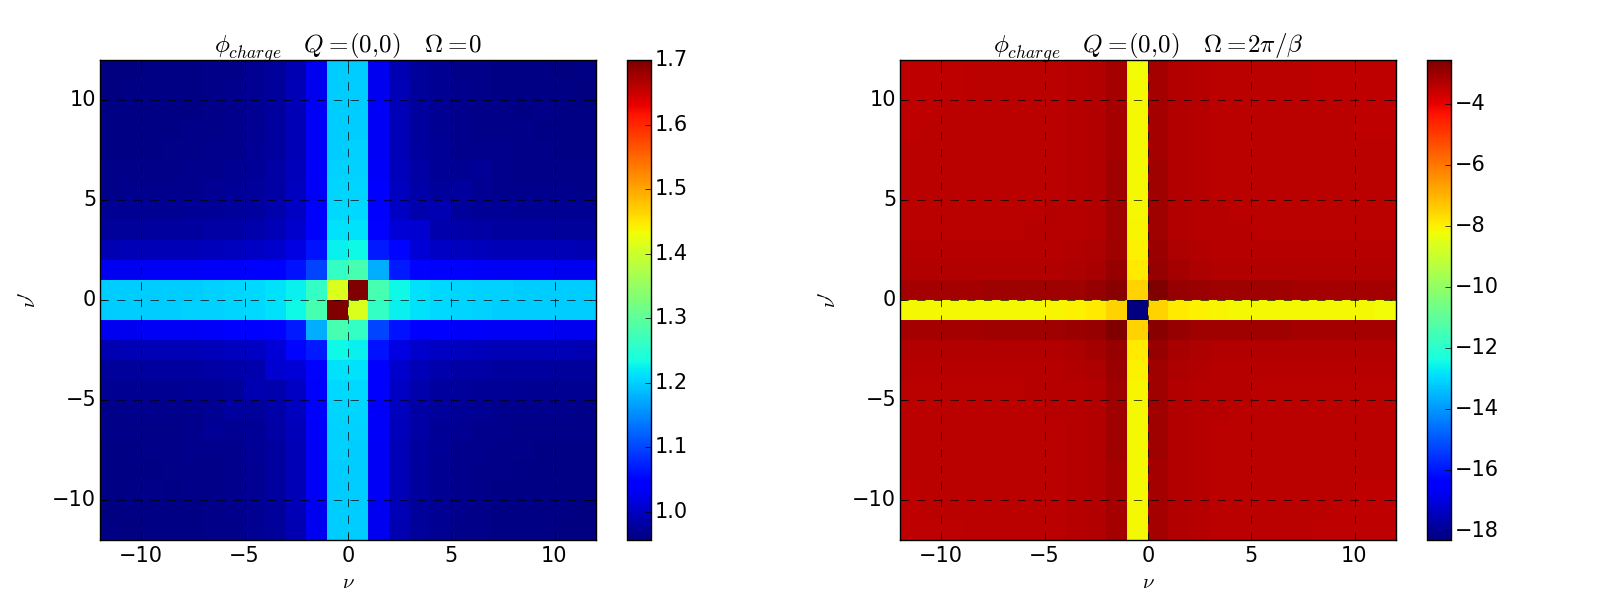
\includegraphics[scale=0.25]{images/Perp_ladder_density.png}
\caption{Charge channel calculated with RPA method for $\Omega=0$ (left) and $\Omega=2\pi/\beta$ (right). }
 \label{Perpladder}
\end{figure}

\begin{figure}
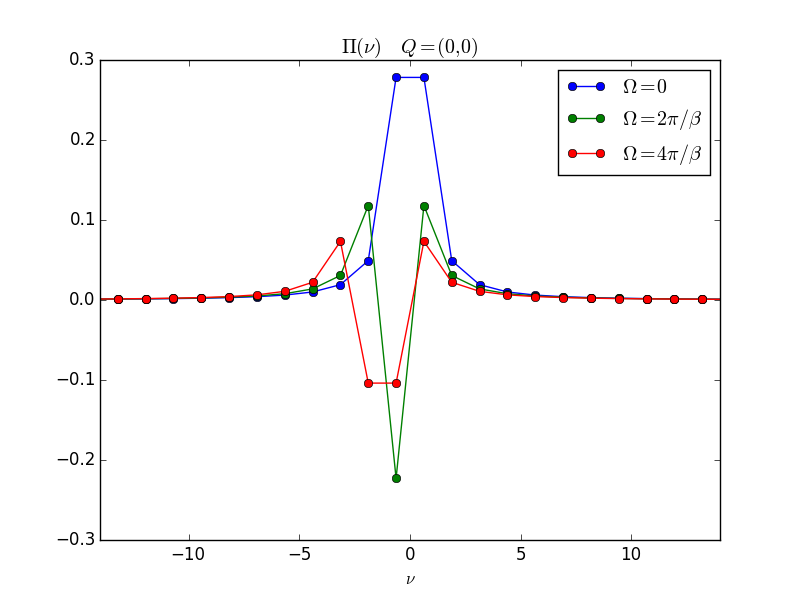
\includegraphics[scale=0.7]{images/Bubble_ph.png}
\caption{PH Bubble as a function of fermionic frequency $\nu$ at $\boldsymbol{Q}=(0,0)$. }
 \label{Perpladder}
\end{figure}